\documentclass[tikz,border=8pt]{standalone}
\usepackage[T1]{fontenc}\usepackage{lmodern}\usetikzlibrary{arrows.meta,positioning}
\begin{document}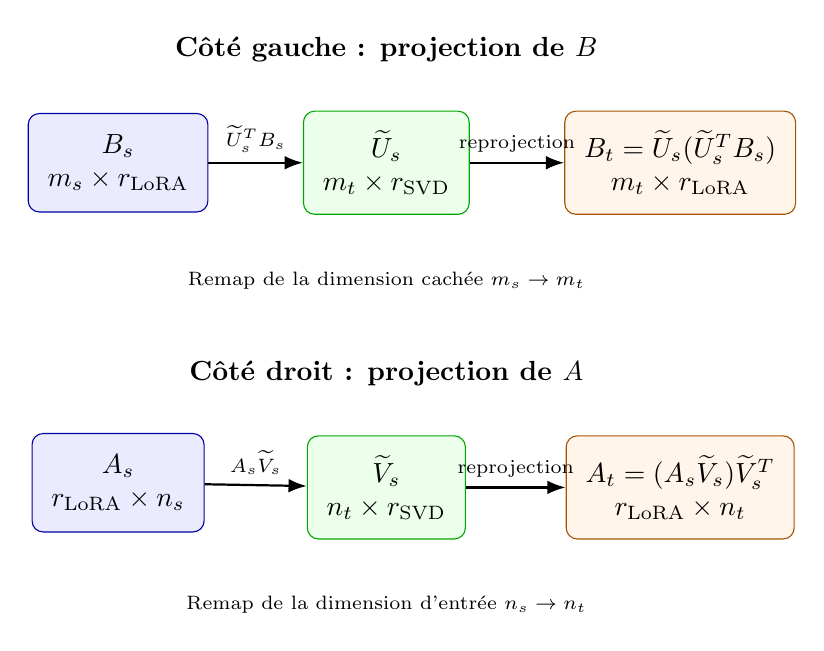
\begin{tikzpicture}[font=\sffamily,>=Latex,box/.style={draw=#1!65!black,fill=#1!8,rounded corners,minimum height=1.25cm,align=center,inner sep=7pt},arr/.style={-{Latex},thick}]
\node[box=blue] (bs) {$B_s$\\$m_s\times r_{\rm LoRA}$};\node[box=green,right=12mm of bs] (u) {$\widetilde U_s$\\$m_t\times r_{\rm SVD}$};\node[box=orange,right=12mm of u] (bt) {$B_t=\widetilde U_s(\widetilde U_s^TB_s)$\\$m_t\times r_{\rm LoRA}$};
\draw[arr] (bs)--node[above,font=\scriptsize]{$\widetilde U_s^TB_s$} (u);\draw[arr] (u)--node[above,font=\scriptsize]{reprojection} (bt);
\node[above=5mm of u,font=\bfseries] {Côté gauche : projection de $B$};\node[below=6mm of u,font=\scriptsize] {Remap de la dimension cachée $m_s\to m_t$};
\node[box=blue,below=28mm of bs] (as) {$A_s$\\$r_{\rm LoRA}\times n_s$};\node[box=green,below=28mm of u] (v) {$\widetilde V_s$\\$n_t\times r_{\rm SVD}$};\node[box=orange,below=28mm of bt] (at) {$A_t=(A_s\widetilde V_s)\widetilde V_s^T$\\$r_{\rm LoRA}\times n_t$};
\draw[arr] (as)--node[above,font=\scriptsize]{$A_s\widetilde V_s$} (v);\draw[arr] (v)--node[above,font=\scriptsize]{reprojection} (at);
\node[above=5mm of v,font=\bfseries] {Côté droit : projection de $A$};\node[below=6mm of v,font=\scriptsize] {Remap de la dimension d'entrée $n_s\to n_t$};
\end{tikzpicture}\end{document}
